\documentclass[conference]{IEEEtran}
\IEEEoverridecommandlockouts
% The preceding line is only needed to identify funding in the first footnote. If that is unneeded, please comment it out.
\usepackage{cite}
\usepackage{amsmath,amssymb,amsfonts}
\usepackage{algorithmic}
\usepackage{graphicx}
\usepackage{textcomp}
\usepackage{xcolor}
\def\BibTeX{{\rm B\kern-.05em{\sc i\kern-.025em b}\kern-.08em
    T\kern-.1667em\lower.7ex\hbox{E}\kern-.125emX}}
\begin{document}

\title{Steam Store Games Exploratory Data Analysis\\}

\author{\IEEEauthorblockA{Hazar Belge}
Galatasaray University, Computer Engineering\\
Istanbul, Turkey \\
Introduction to Data Analysis}

}

\maketitle


\section{Introduction}
	Steam is a video game digital distribution service by Valve. It was launched as a standalone software client in September 2003 as a way for Valve to provide automatic updates for their games and, expanded to include games from third-party publishers. Steam has also expanded into an online web-based and mobile digital storefront. 


	In this paper, we will look into a dataset about different video games with their different attributes like price, owner count, playtime, achievements count etc.

	After having introduced the data throughly we will ask a research question and technical questions to help answer it. In the end we will have an explanation of the methods we predict on using to answer the questions that we previously posed.\\

\section{Questions about our data}
To analyse our data, first we need a high level question. Upon our introduction of the dataset, we have a much clearer picture regarding what we can focus on.

\subsection{The High Level Question: What are the attributes that affect game sales the most?}\label{AA}
While developing video games, the sales numbers of the game and the income we can generate from it are very important. That's why we want our game to sell well, but it is not certain what are the attributes that make this sale big. There are many factors that will affect game sales. While Flappy Bird with almost no budget makes millions, the game with a budget of millions of dollars may not be liked at all and may not make a profit. Which brings us to our high-level research question that may reveal the solution to this problem. “What are the attributes that affect game sales the most? Of course, we also need subquestions to answer this question.

\subsection{Sub Questions}
\begin{itemize}
\item Does having more reviews achievements affects the game sales positively?
\item Do higher age ratings affect the game sales negatively?
\item Does having english support affects the game sales positively?
\item Do genres affect the game sales?
\item Do categories affect the game sales?
\item Does developers' name affects the game sales?
\item Does having more platform support affects the game sales positively?
\item Do higher prices affect the game sales negatively?
\item Does publishers' name affects the game sales?
\item Do release dates affect the game sales?
\item Does having more reviews affects the game sales positively?
\end{itemize}

\section{Steam Dataset}
This dataset is published by Nik Davis on Kaggle. It includes 27075 different video games and 18 different attributes for each of them from Steam. The dataset was last updated in May 2019, so I removed the games that were released in 2019 to prevent them from misleading the year-to-year comparison. After this removing process we have 24862 video games in total. So, let's take a look at some of attributes of dataset.

\subsection{Achievements}


\begin{figure}[htp]
  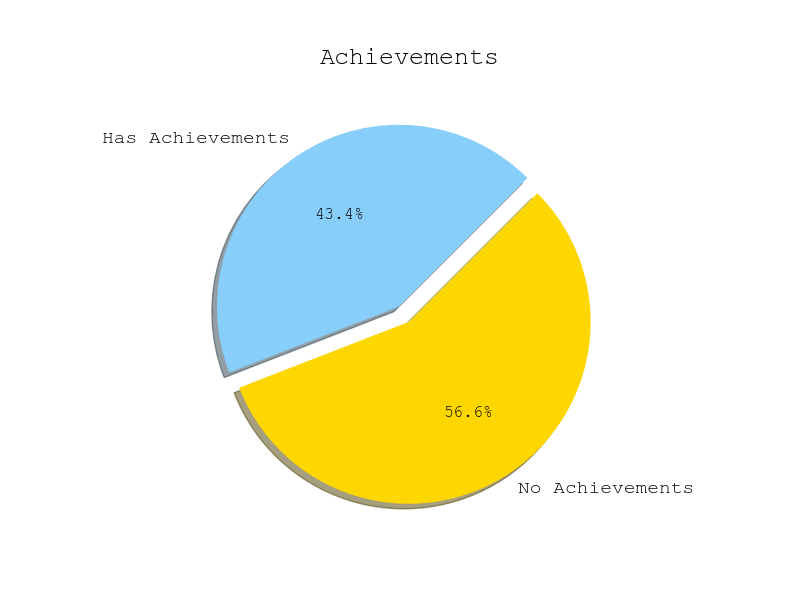
\includegraphics[width=\linewidth]{assets/achievements_pie.png}
  \caption{How many games have achievements?}
  \label{fig:achievements1}
\end{figure}

\begin{figure}[htp]
  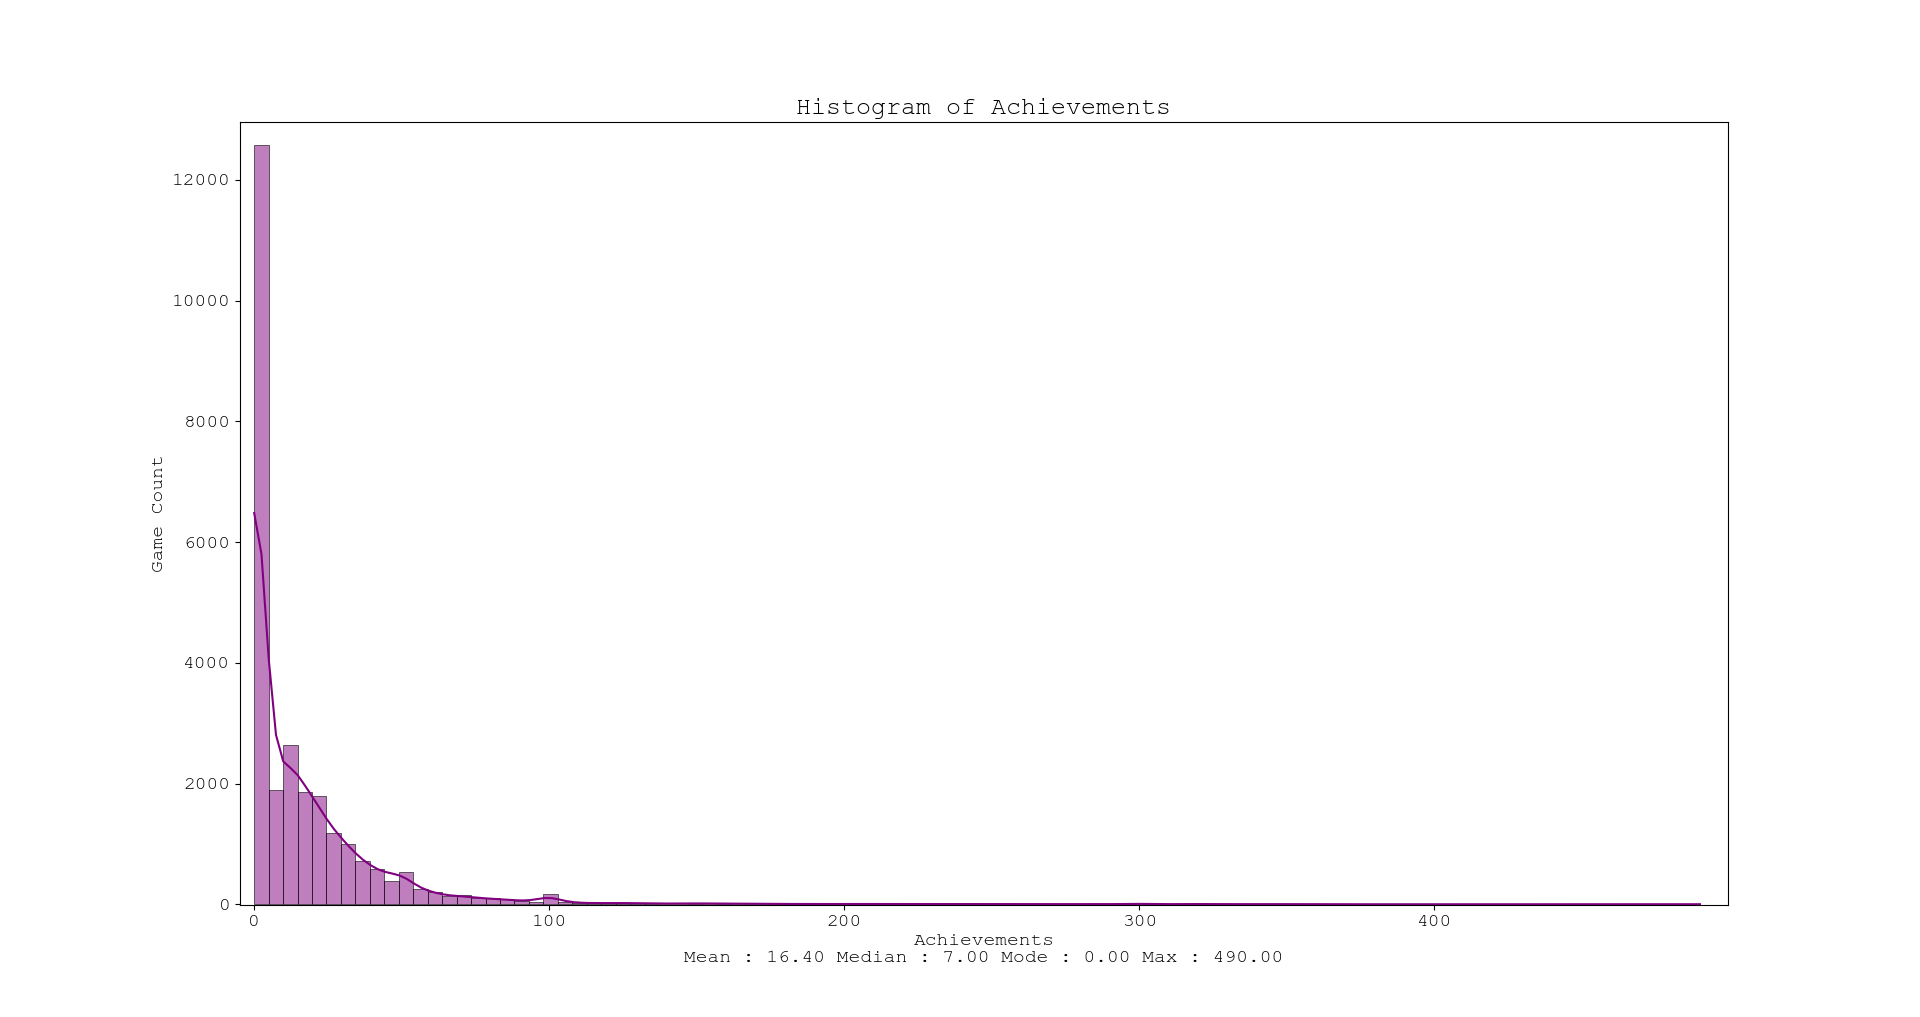
\includegraphics[width=\linewidth]{assets/achievements_hist.png}
  \caption{Histogram of Achievements.}
  \label{fig:achievements2}
\end{figure}


\subsection{Age Rating}


\begin{figure}[h]
  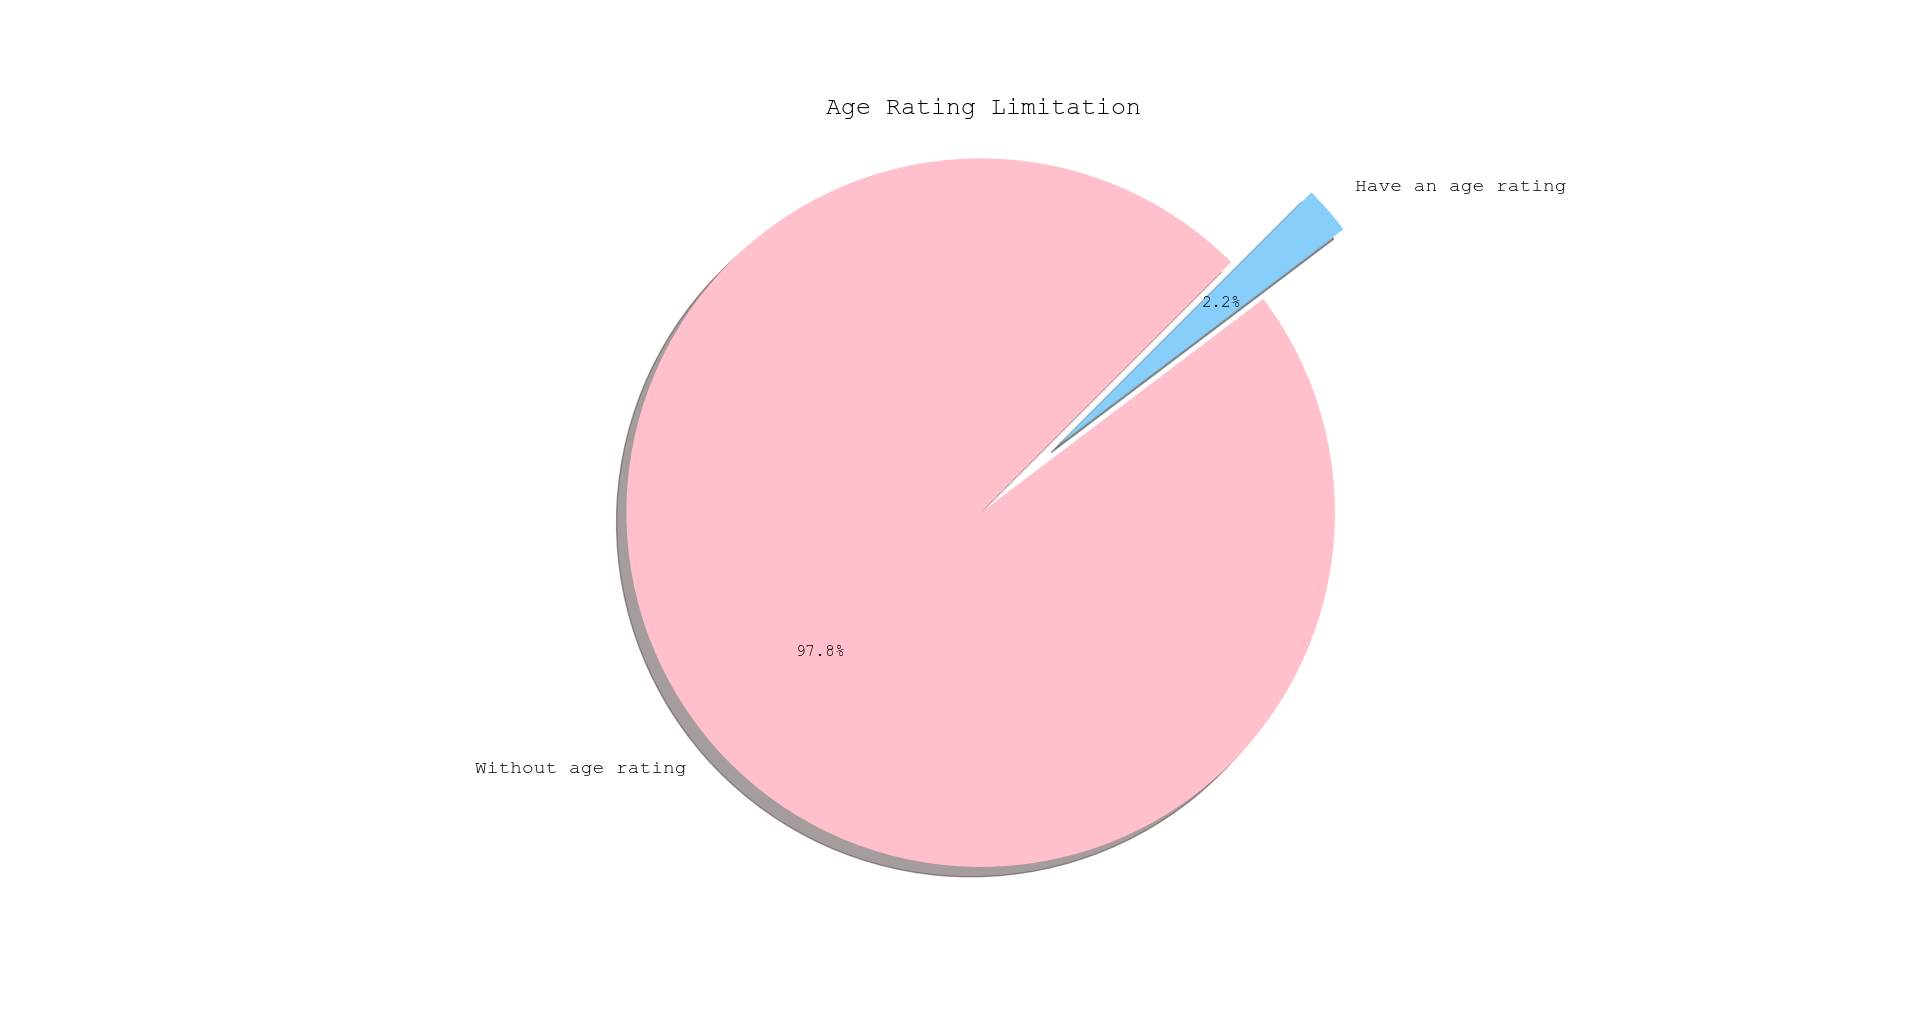
\includegraphics[width=\linewidth]{assets/age_rating_pie.png}
  \caption{How many games have age rating?}
  \label{fig:agerating1}
\end{figure}


\begin{figure}[h]
  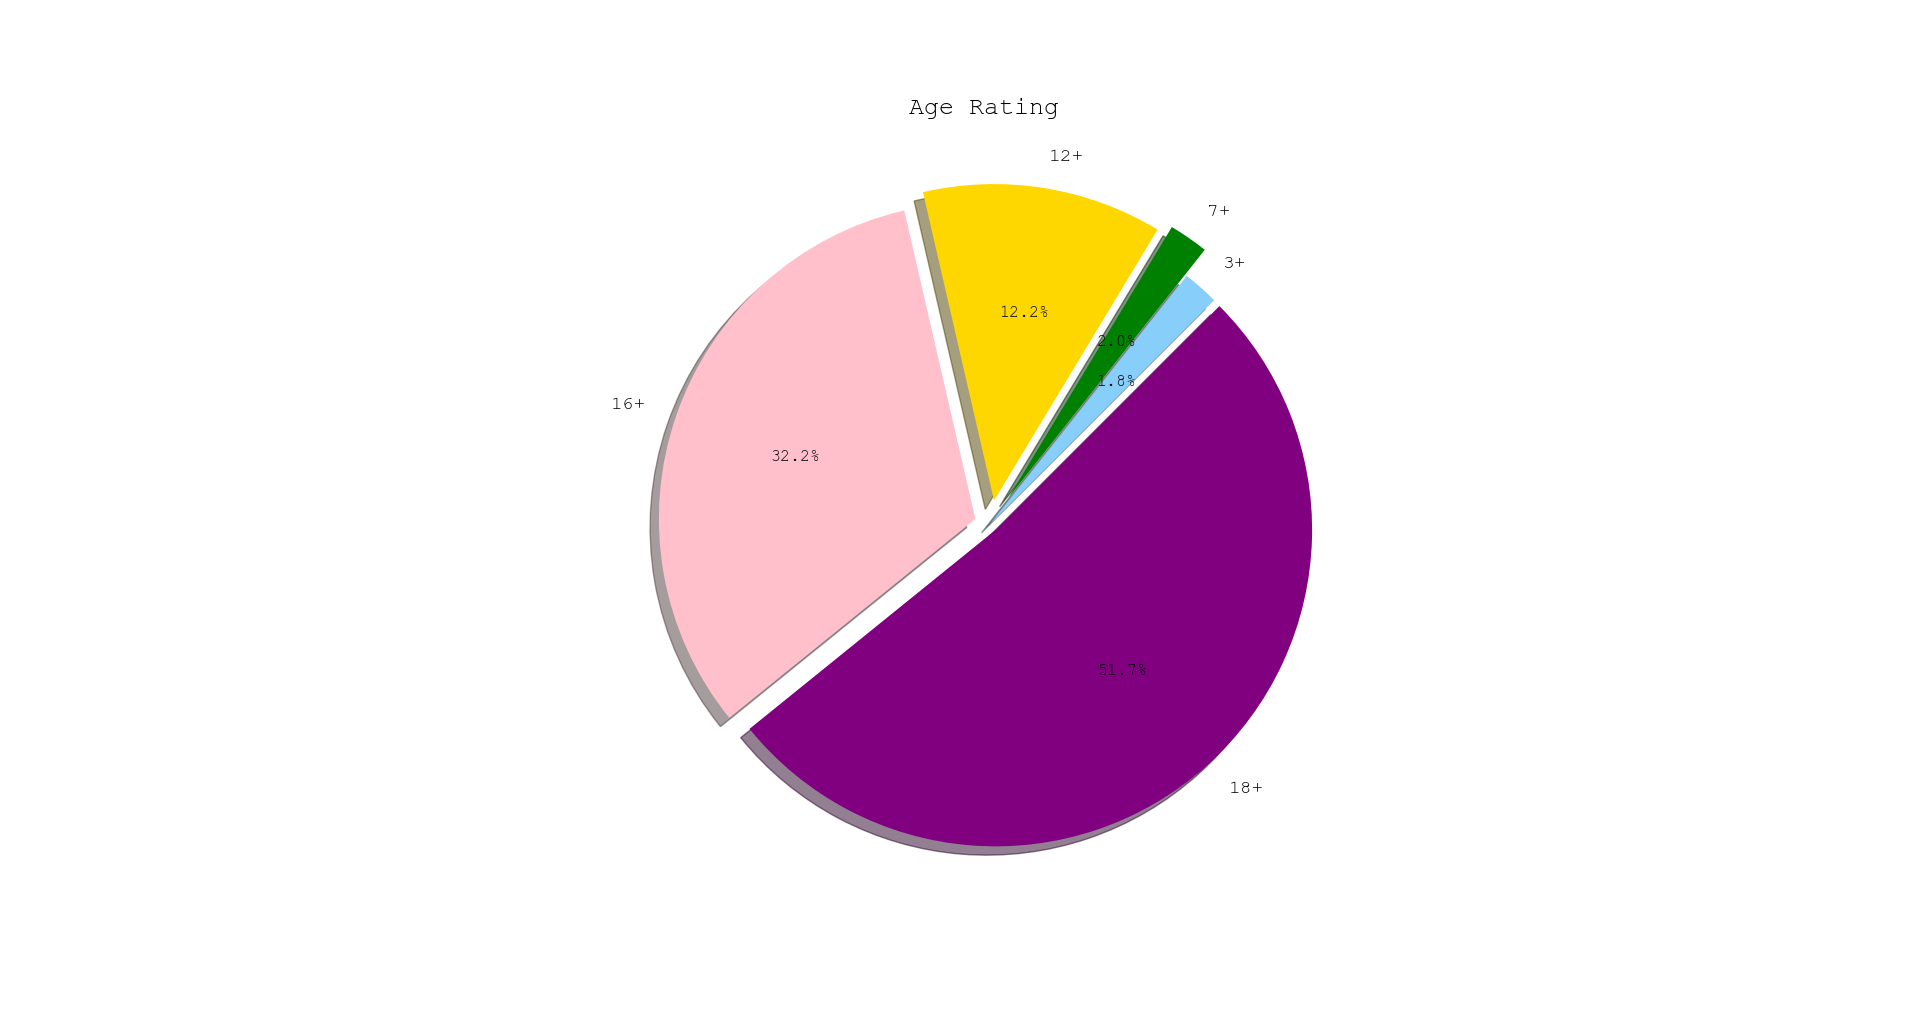
\includegraphics[width=\linewidth]{assets/age_rating_has_pie.png}
  \caption{Age Ratings Pie Chart.}
  \label{fig:agerating2}
\end{figure}


\subsection{Category}


\begin{figure}[h]
  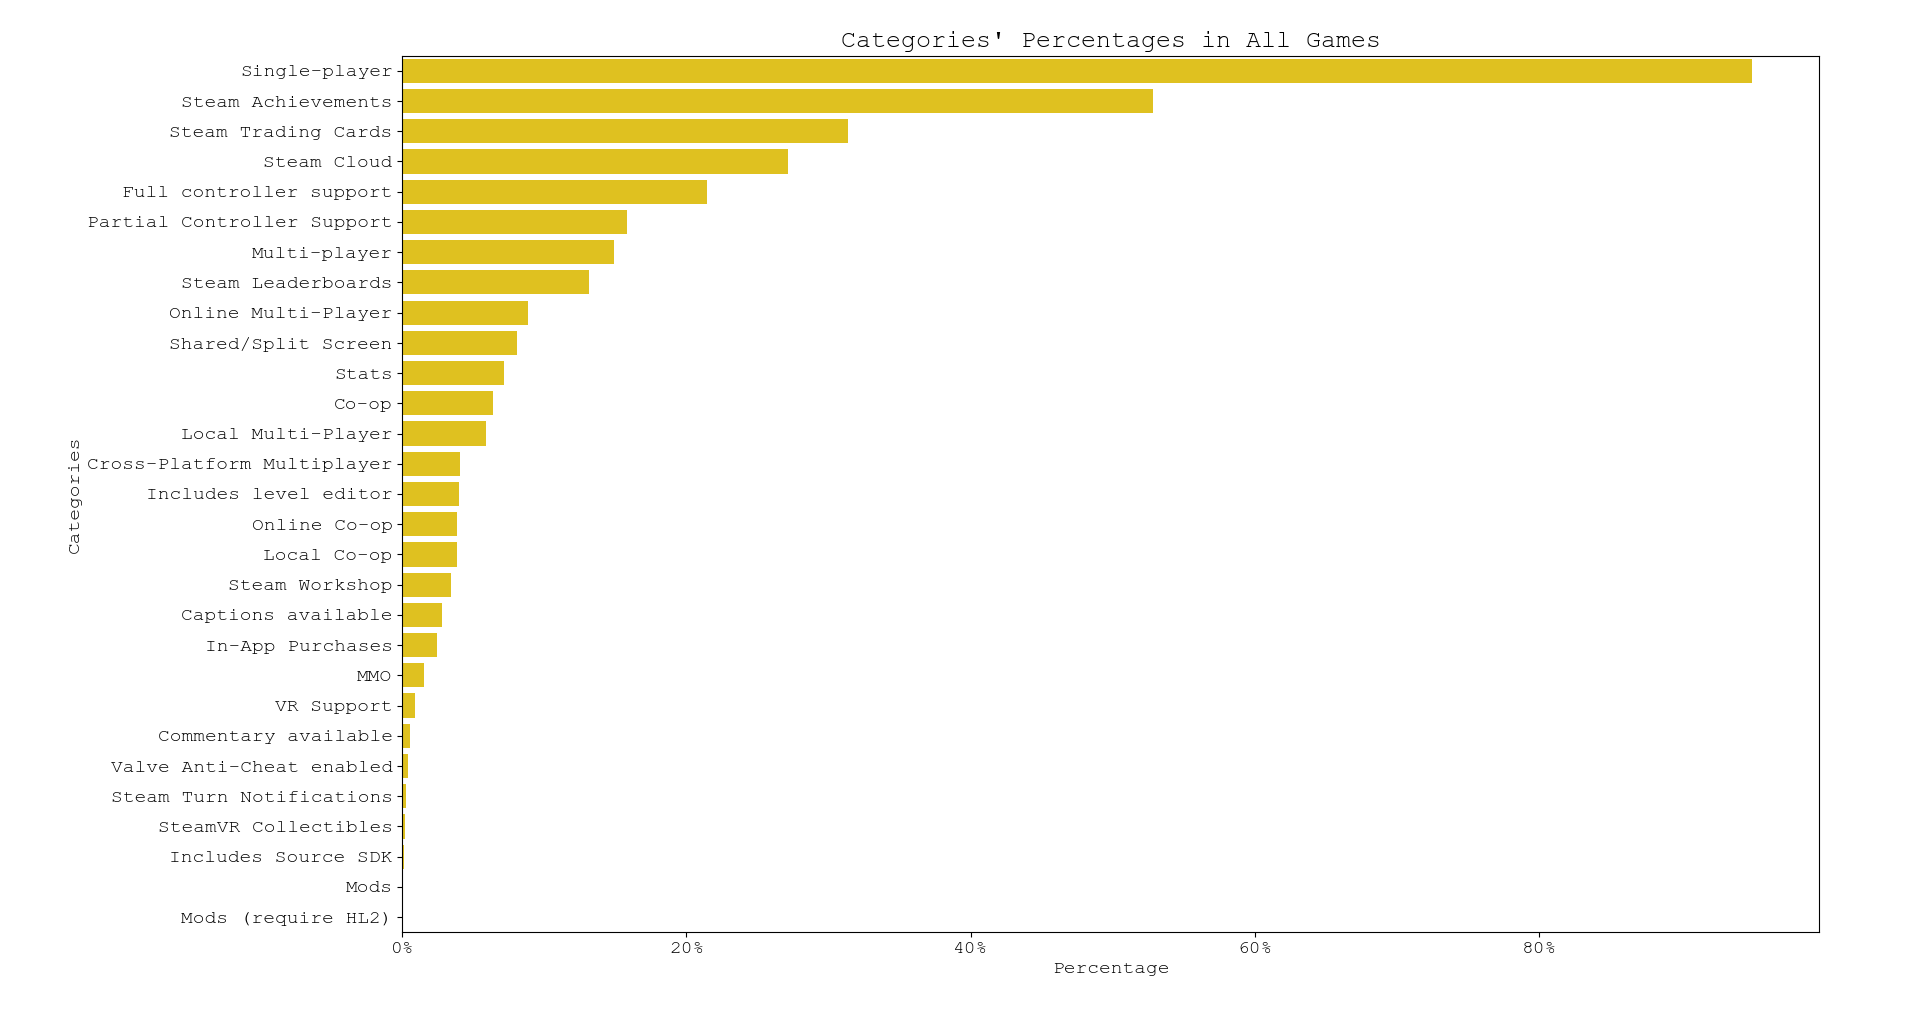
\includegraphics[width=\linewidth]{assets/categories_dist.png}
  \caption{Categories' percentages of all games.}
  \label{fig:category1}
\end{figure}


\subsection{English Support}


\begin{figure}[h]
  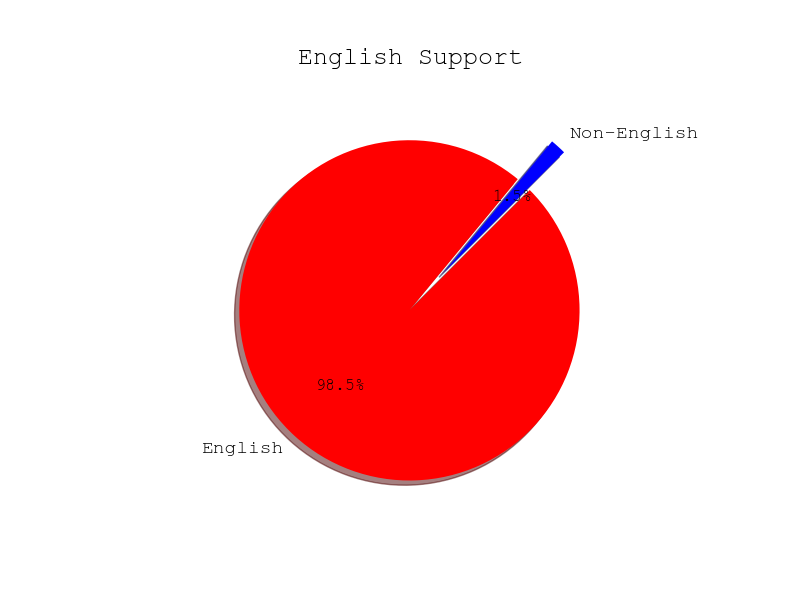
\includegraphics[width=\linewidth]{assets/english_support_pie.png}
  \caption{How many games have English support?}
  \label{fig:englishsupport1}
\end{figure}


\subsection{Genre}


\begin{figure}[h]
  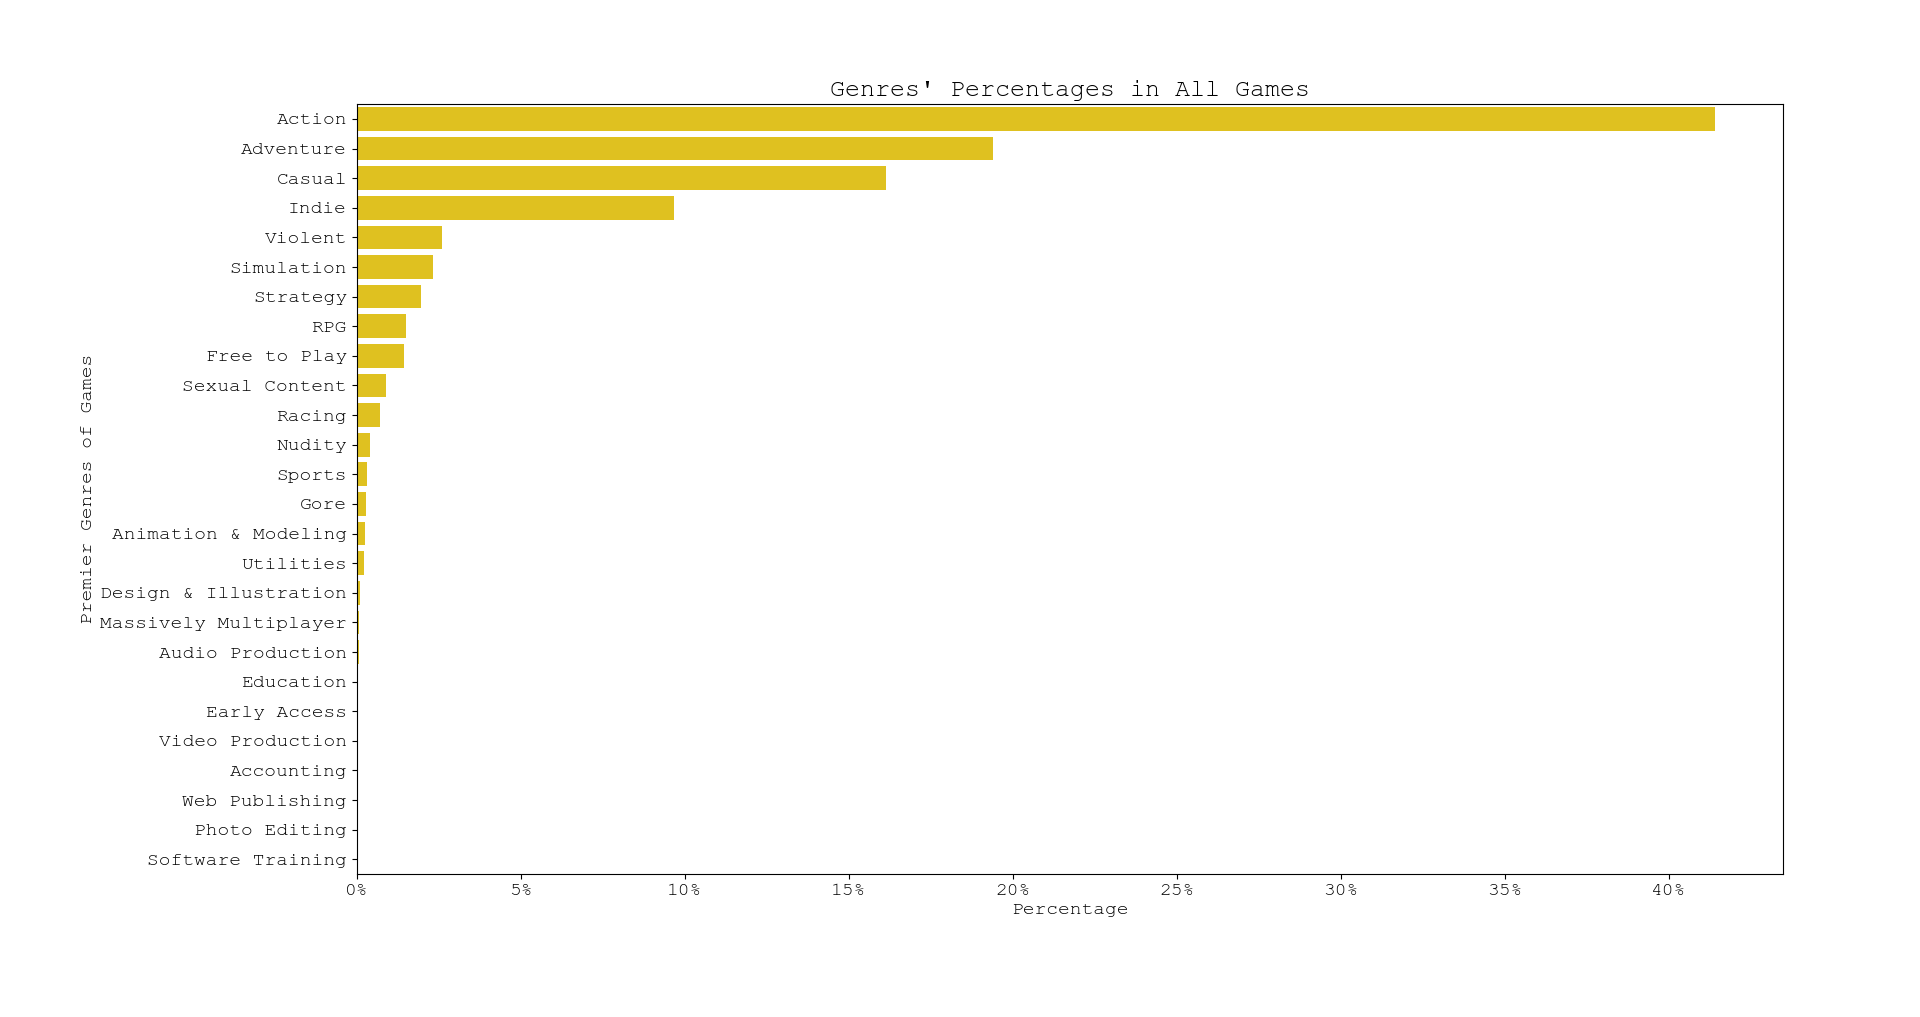
\includegraphics[width=\linewidth]{assets/genres_dist.png}
  \caption{Genres' percentages of all games.}
  \label{fig:genre1}
\end{figure}


\subsection{Owner Count}


\begin{figure}[h]
  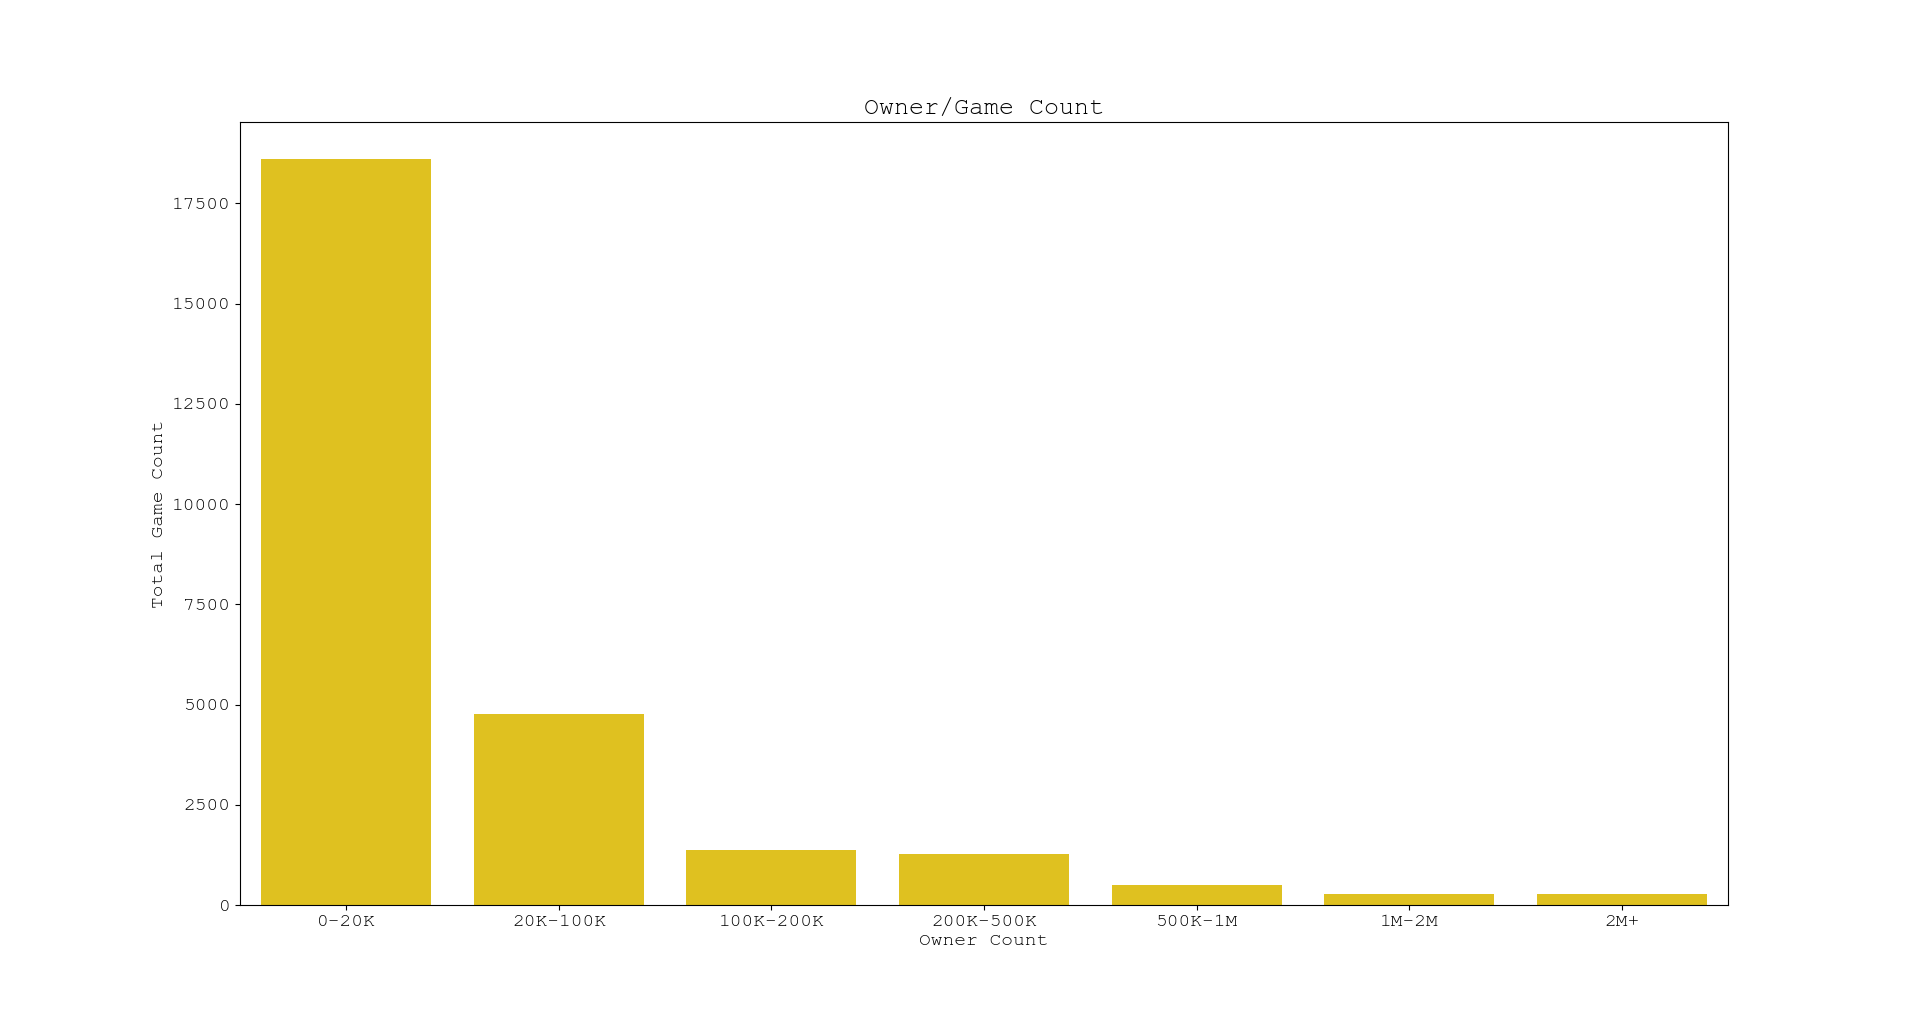
\includegraphics[width=\linewidth]{assets/owners_count.png}
  \caption{Distribution of owners count in all games.}
  \label{fig:ownercount1}
\end{figure}


\subsection{Platform}


\begin{figure}[h]
  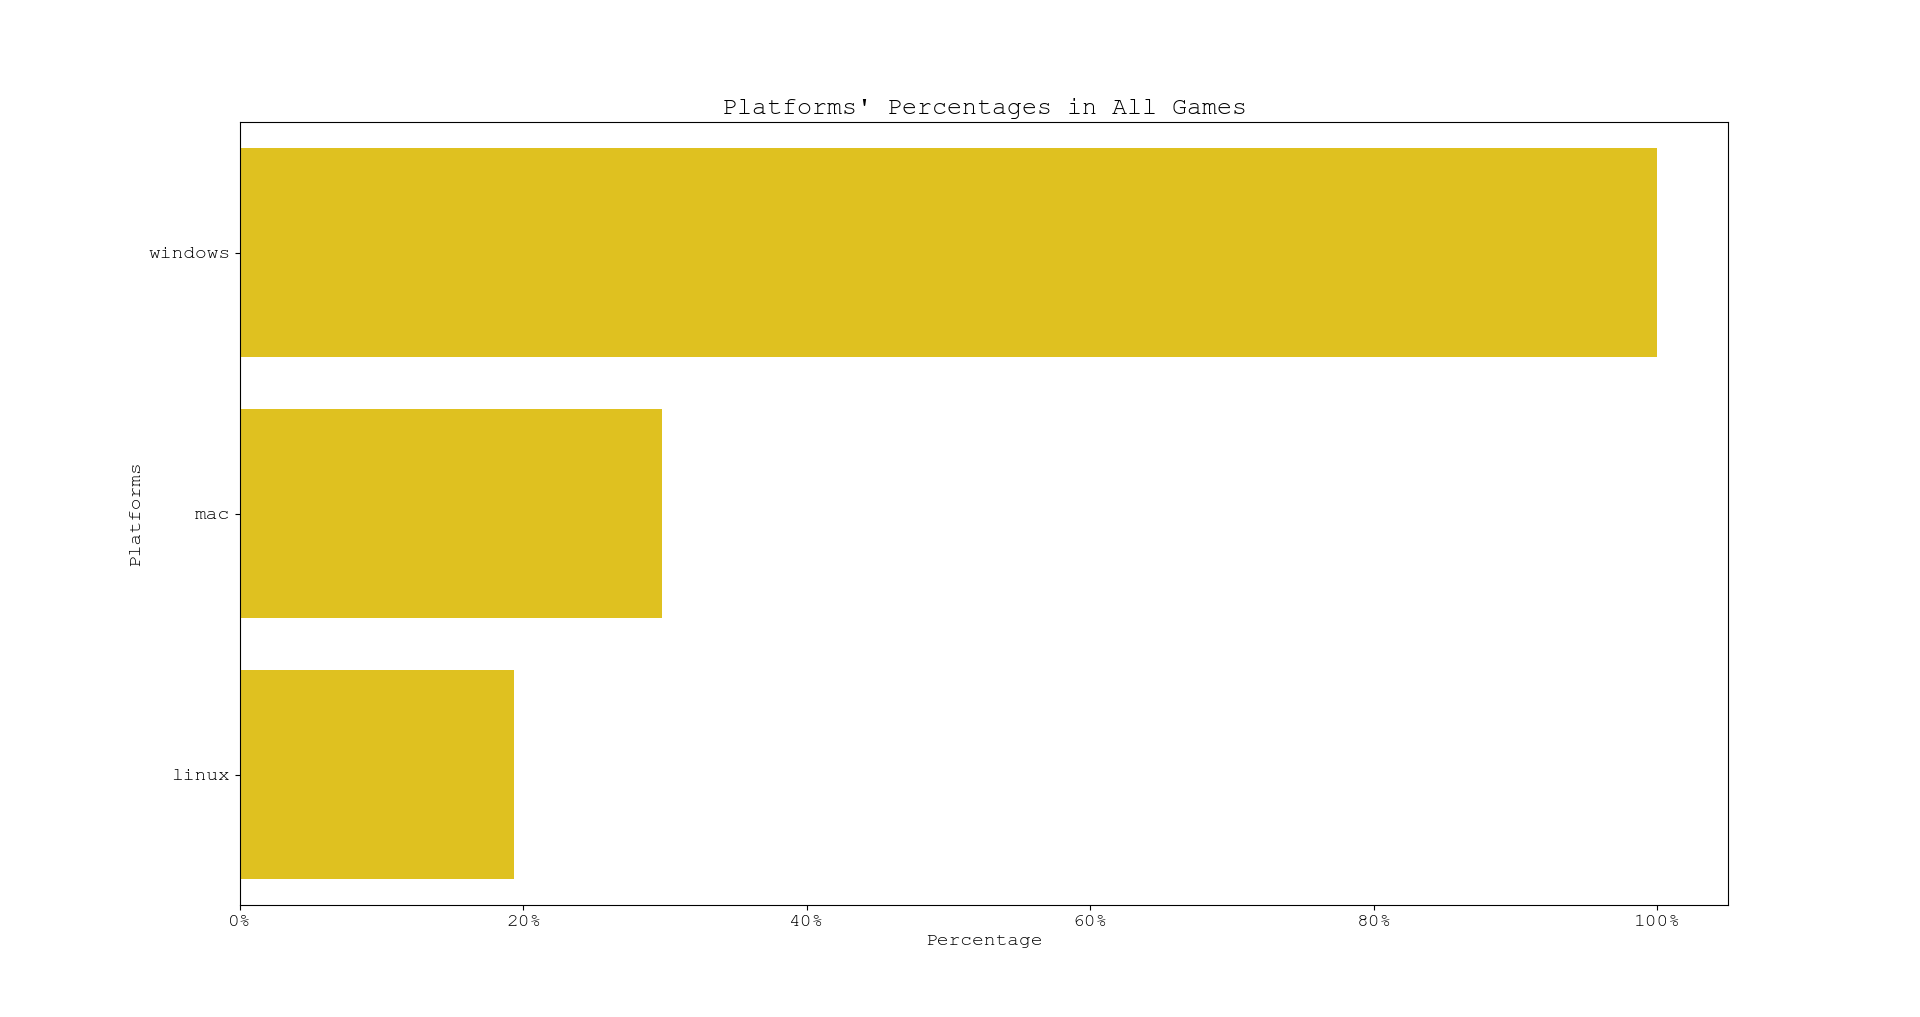
\includegraphics[width=\linewidth]{assets/platforms_dist.png}
  \caption{Platforms' percentages of all games.}
  \label{fig:platform1}
\end{figure}


\subsection{Positive Rate}


\begin{figure}[h]
  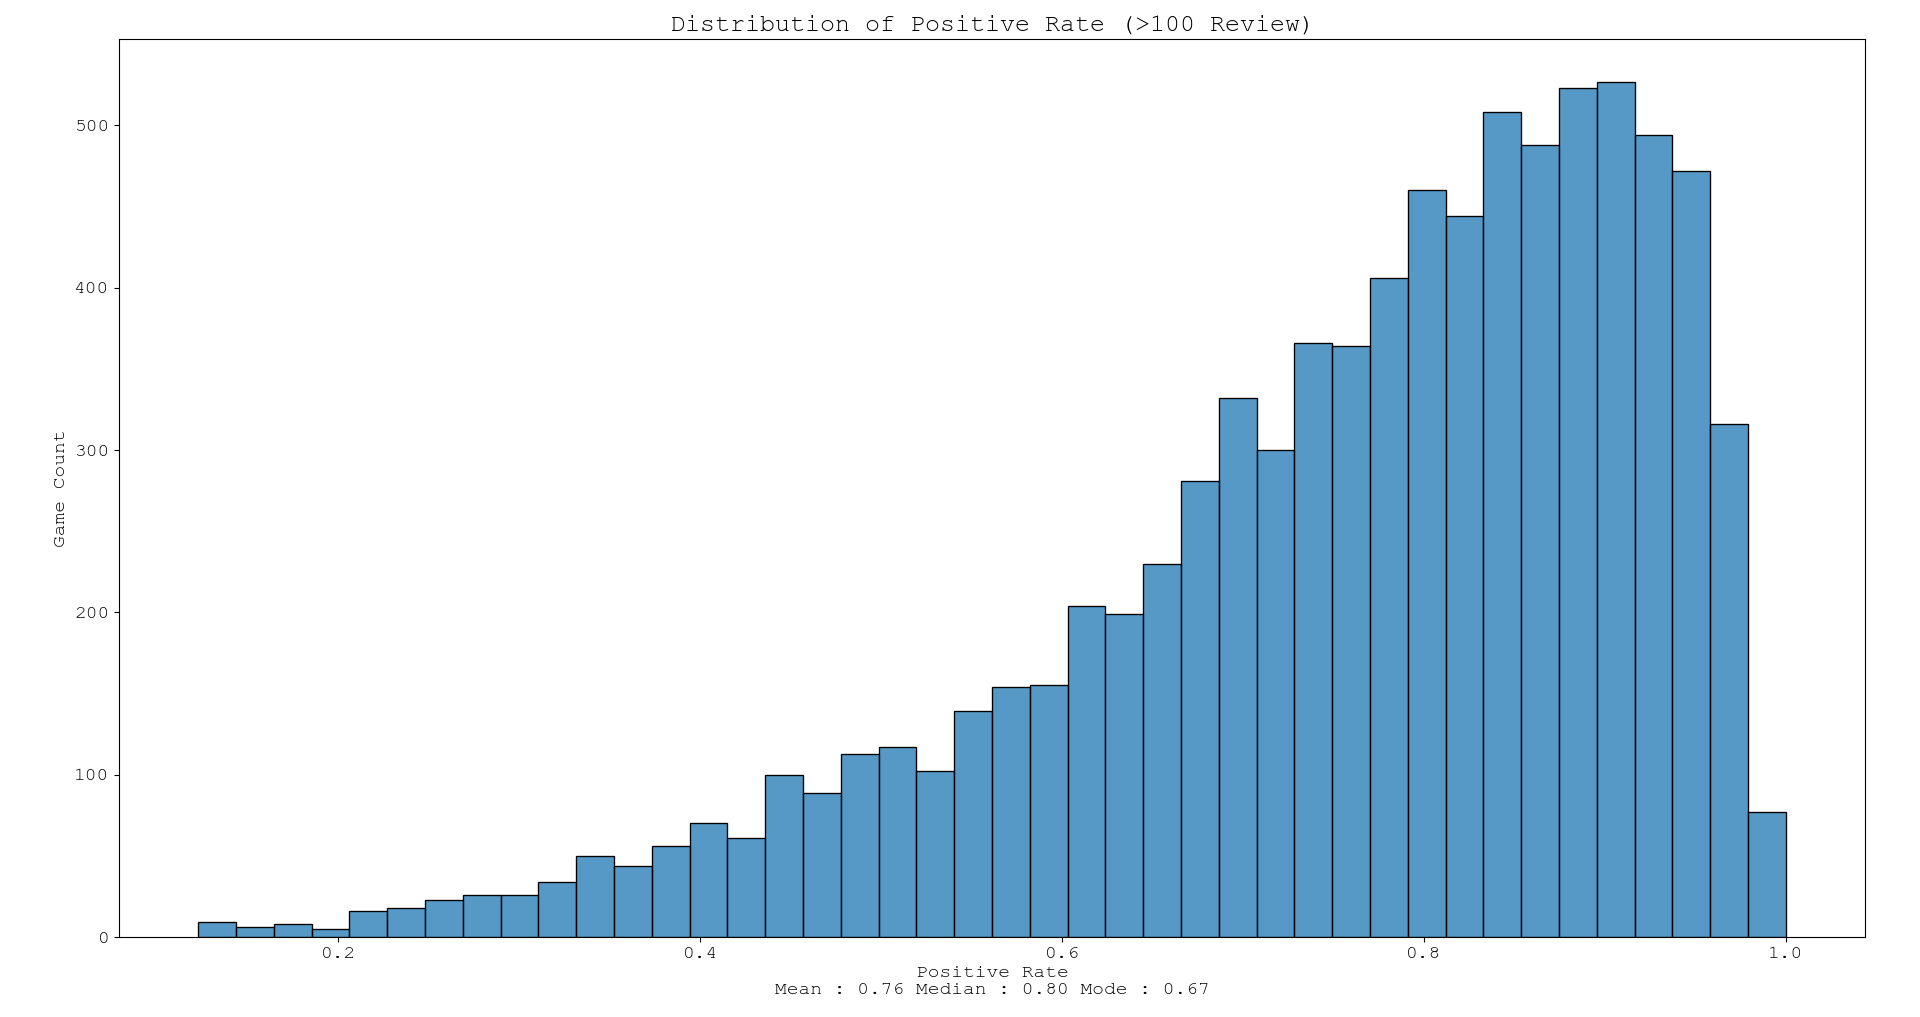
\includegraphics[width=\linewidth]{assets/positive_rate_dist.png}
  \caption{Histogram of Positive Rate.}
  \label{fig:positiverate1}
\end{figure}


\subsection{Price}


\begin{figure}[h]
  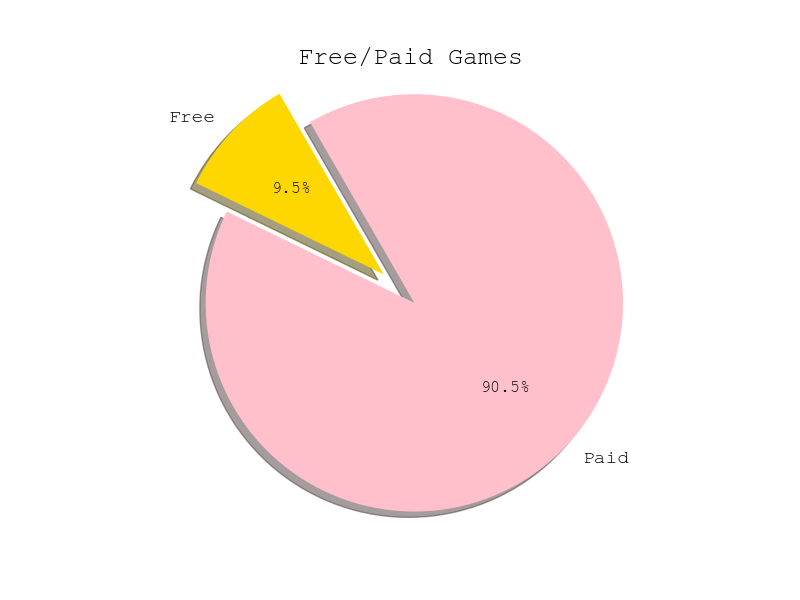
\includegraphics[width=\linewidth]{assets/price_free_paid_pie.png}
  \caption{How many games are paid?}
  \label{fig:price1}
\end{figure}

\begin{figure}[h]
  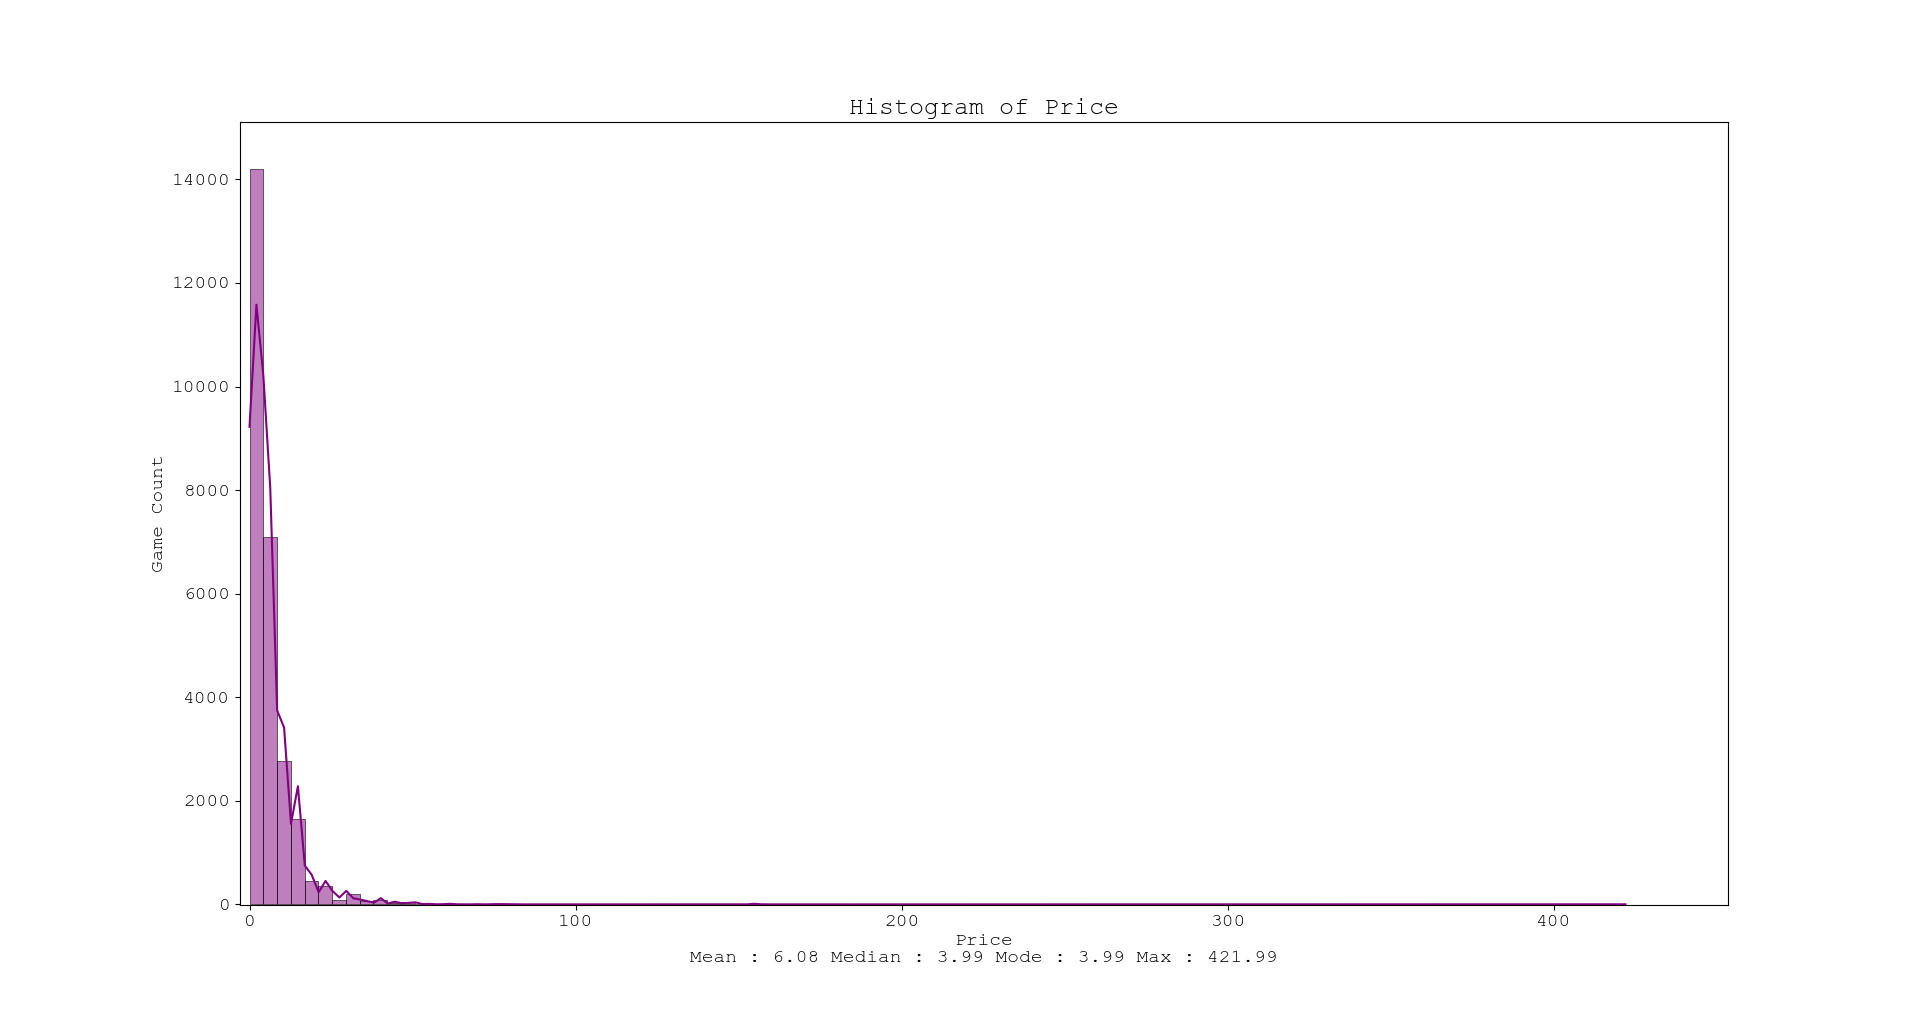
\includegraphics[width=\linewidth]{assets/price_hist.png}
  \caption{Histogram of Price.}
  \label{fig:price2}
\end{figure}

\subsection{Released Date}


\begin{figure}[h]
  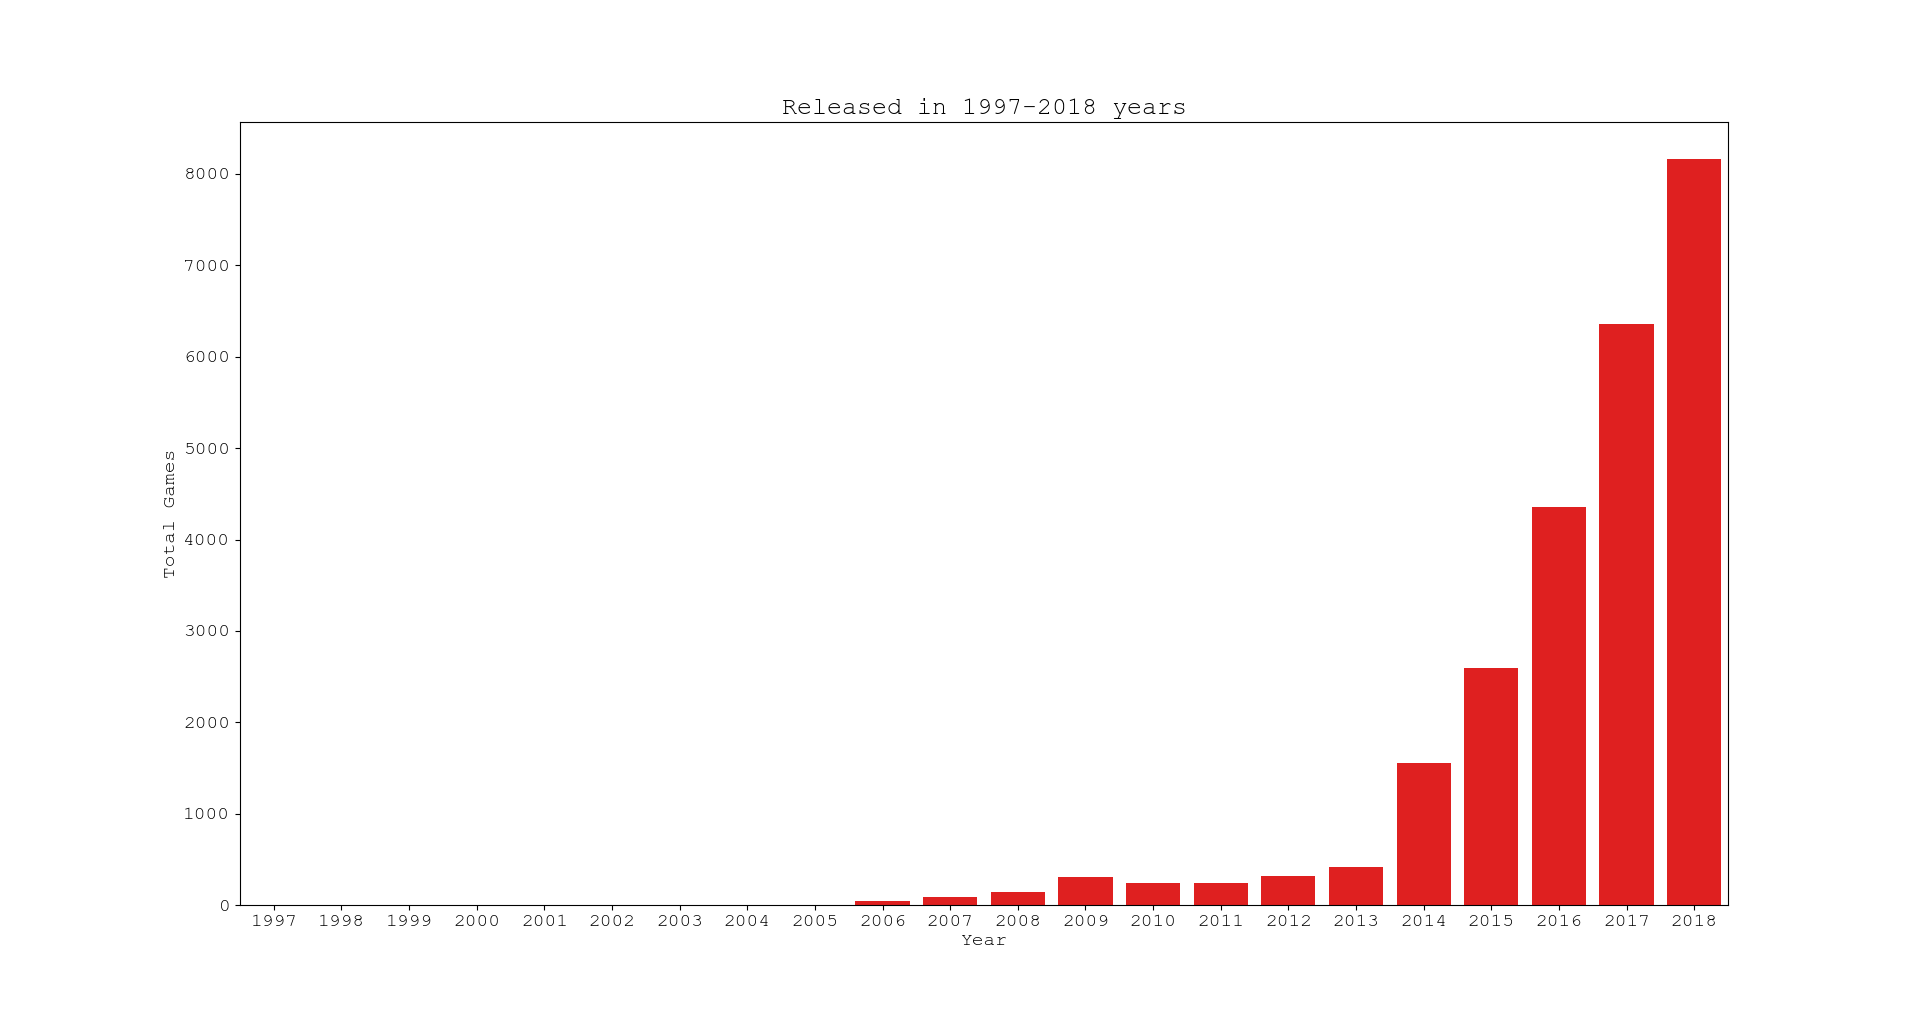
\includegraphics[width=\linewidth]{assets/released_date_bar.png}
  \caption{Video Games Per Year.}
  \label{fig:releaseddate1}
\end{figure}


\section{Constructing Hypothesis Tests And The
Methods}

\end{document}
